%\begin{frame}{Salient Characteristics for Deciding to Intervene}
%\begin{itemize}
%\item Model the environment as a STRIPS style planning domain
%\item Use an automated planner to sample plans for the undesirable states
%\end{itemize}
%	\begin{figure}[t]
%		\centering{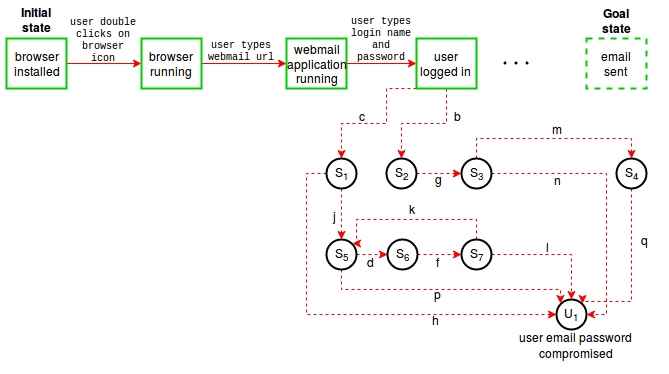
\includegraphics[width=0.7\columnwidth]{states.png}}
%	\end{figure}
%Observation trace\\ $[$\texttt{{\small user double clicks on browser icon, user types webmail url, user types login name and password}}$]$
%
%\end{frame}


\begin{frame}{Salient Characteristics for Deciding to Intervene}
	\begin{itemize}
		\item Certainty (C)
		\begin{itemize}
			\item How many plans contained the action over the number of sampled plans
			\item Highlight frequently occurring actions in plans as important
		\end{itemize}
		
		\item Timeliness (T)
			\begin{itemize}
				\item Maximum normalized steps remaining in the sampled plans
				\item Quantifies how soon the undesirable state may occur
			\end{itemize}
		
		\item Desirability (D)	
		\begin{itemize}
			\item Number of times the action appears in the sampled plans over the sum of actions in the sampled plans
			\item Separate common harmless actions that further the user’s actual goal from harmful actions to be avoided
			\item Negative metric
		\end{itemize}
		
	\end{itemize}
\end{frame}


\begin{frame}{Undesirable Consequences Recognition Function}
	\begin{itemize}
	\item Critical Trigger Action is an observed action that maximizes $V(a)$:
	
		\begin{align*}
		V(a) &= \alpha_1 * Certainty (a|\Pi_U) +\;\alpha_2 * Timeliness (a|\Pi_U) \\ &-\;\alpha_3 * Desirability (a|\Pi_U)
		\end{align*}
		
		\item $a  $ candidate action from the sampled undesirable plans plans
		\item $\Pi_U  $ sampled undesirable plans
		\item $(\alpha_1, \alpha_2, \alpha_3)  $ metric weight assignments
	\end{itemize}

\end{frame}